\documentclass[10pt]{beamer}

\usetheme{Boadilla}

\usepackage{pgf}
\usepackage[english]{babel}
\usepackage[utf8]{inputenc}

\usepackage{bm}
\usepackage{tikz}

\usepackage{times}
\usepackage[T1]{fontenc}

\definecolor{basecolor}{RGB}{79, 17, 32}

\title[\pgfuseimage{department-logo}] %
{A Markov model for automatic segmentation in audio recodings}

\author[Rafael de Jesús Robledo Juárez] %
{Rafael de Jesús Robledo Juárez \\
\small{\texttt{rrobledo@cimat.mx}} \\ ~\\
\small{Advisor: Salvador Ruíz-Correa Ph.D}}


\institute[CIMAT]
{
  Computer Science Department\\
  Center for Mathematical Research (CIMAT), Guanajuato \\
  ~ \\
  \pgfuseimage{university-logo}
}

\date[February 2013]
{Preliminary thesis presentation, 2013}
\subject{Latex Beamer Template}

\pgfdeclareimage[interpolate=true, height=2.5cm]{university-logo}{logos/logo-big}
\pgfdeclareimage[interpolate=true, height=0.6cm]{department-logo}{logos/logo-trans}
%\logo{\pgfuseimage{department-logo}}

\usecolortheme[named=basecolor]{structure} 
\setbeamertemplate{navigation symbols}{} 

\begin{document}

\newcommand*\actwidth{8cm}
\newcommand*\actheight{1.6em}

\tikzset{entry/.style 2 args={
    xshift=(0.5334em+0.8pt)/2,
    draw,
    font=\sffamily,
    rectangle,
    rounded corners,
    fill = basecolor!70,    
    anchor=north west,
    line width=0.1pt,
    inner sep=0.3333em,
    text width={\actwidth/#2-1.2em-1.6pt},
    minimum height=#1*\actheight,
    align=center
}}

\setbeamertemplate{itemize items}[default]
\setbeamertemplate{enumerate items}[default]
\setbeamerfont{section number projected}{series=\bfseries,size={\fontsize{8}{12}}}
\setbeamertemplate{sections/subsections in toc}[square]

\begin{frame}
  \titlepage
\end{frame}

\section{Introduction}

\subsection{Main objectives}

\begin{frame}{Main objectives}
  \begin{itemize}
  	\item
  	  Use a Hidden Markov Model to partitioning an audio recording into similar-speaker regions.
  	  Each segment should correspond to a different speaker.
       
     \item
       This task is known as Speaker diarization. Has two main stages: segmentation and clustering.
       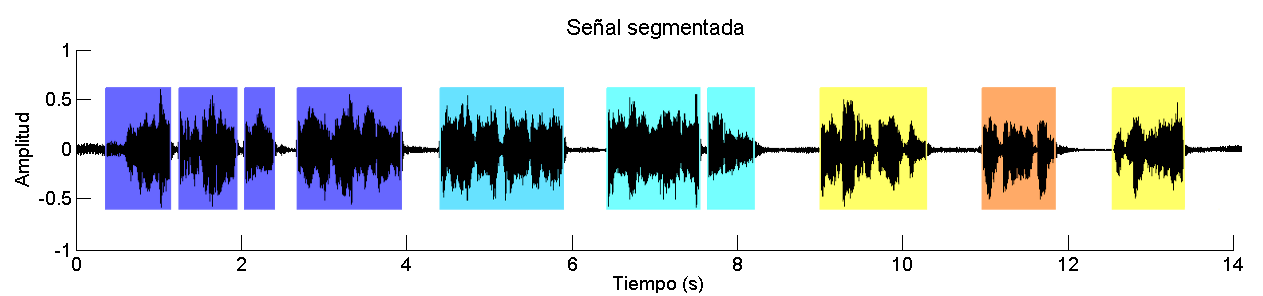
\includegraphics[width=0.9\textwidth]{gfx/f-segm}

  	\item	
       Each of the segments will be labeled according to different speakers found in the conversation.
  \end{itemize}
\end{frame}

\subsection{Motivation}

\begin{frame}{Motivation}
  \begin{itemize}
    \itemsep 2.5em  
    \item Speaker identification in a audio recording it's an important stage 
    for improving results in different NPL applications such as automatic transcription
    and speech recognition, as long as it allow us to fit a model for each different found speaker.

    \item A remarkable point in the automation of this process is to perform segmentation with out needing 
    of priori knowledge on the number or gender of persons involved in recording.   
  \end{itemize}
\end{frame}

\section{Methodology}

\subsection{Signal processing}

\begin{frame}{Methodology}{Signal processing (1)}
\small {
\vspace{0mm} 
\begin{columns}   
  \begin{column}{0.6\textwidth} 
    \hfill  
    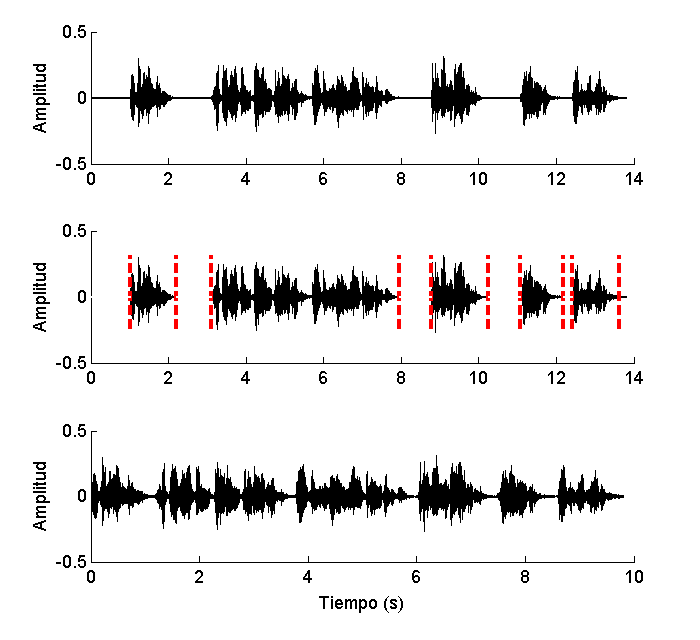
\includegraphics[width=0.9\textwidth]{gfx/filename51}    
  \end{column}
  \begin{column}{0.4\textwidth}
    \vspace{-8mm} 
    \begin{itemize}
      \setlength{\itemindent}{-2em}      
      \itemsep 4.6em    
      \item Original signal
      \item Silence identifier
      \item Truncated signal
    \end{itemize}
  \end{column}   
\end{columns}   
}
\end{frame}

\begin{frame}{Methodology}{Signal processing (2)}
\small {
\vspace{0mm} 
\begin{columns}   
  \begin{column}{0.6\textwidth} 
    \hfill  
    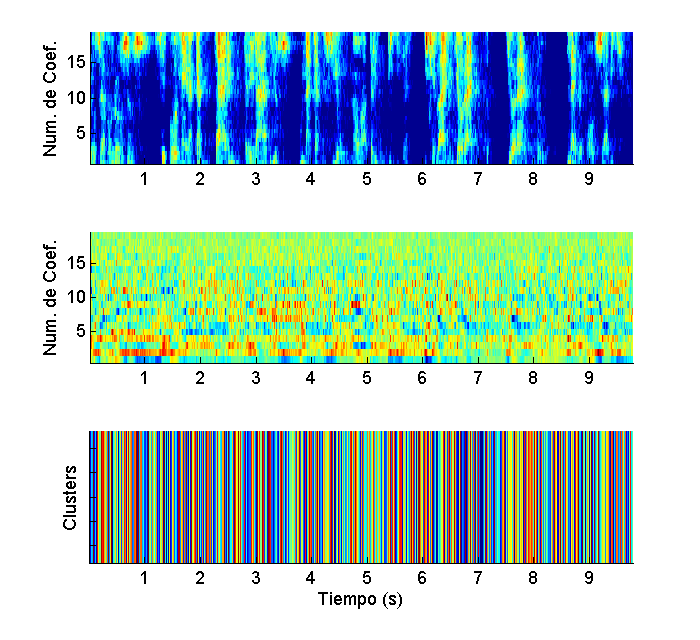
\includegraphics[width=0.9\textwidth]{gfx/filename52}    
  \end{column}
  \begin{column}{0.4\textwidth}
    \vspace{-8mm} 
    \begin{itemize}
      \setlength{\itemindent}{-2em}      
      \itemsep 4.6em    
      \item FFT + Filter Bank
      \item log + DCT
      \item k-means ++
    \end{itemize}
  \end{column}   
\end{columns}   
}
\end{frame}

\subsection{Model}
\begin{frame}{Methodology}{Model}
  \begin{center}
    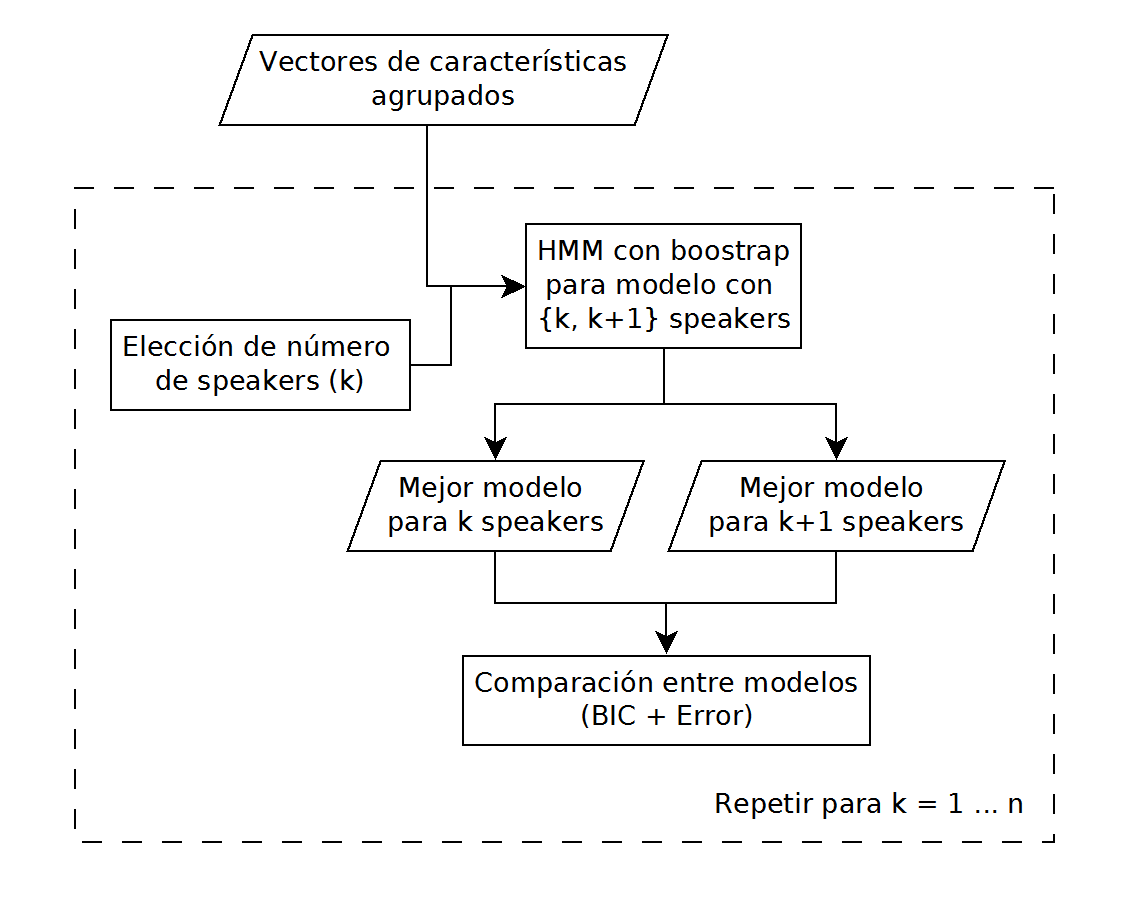
\includegraphics[width=0.7\textwidth]{gfx/dia-hmm}
  \end{center}
\end{frame}

\section{Progress}
\begin{frame}{Progress}
  \begin{itemize}
    \itemsep 3em
    \item System implementation completed.
    \item Results for synthetic data (randomly generated).
    \item Starting tests for synthetic voice recordings.
  \end{itemize}
\end{frame}

\section{Results}
\subsection{Synthetic data tests}
\begin{frame}{Synthetic data tests}
  \begin{center}
    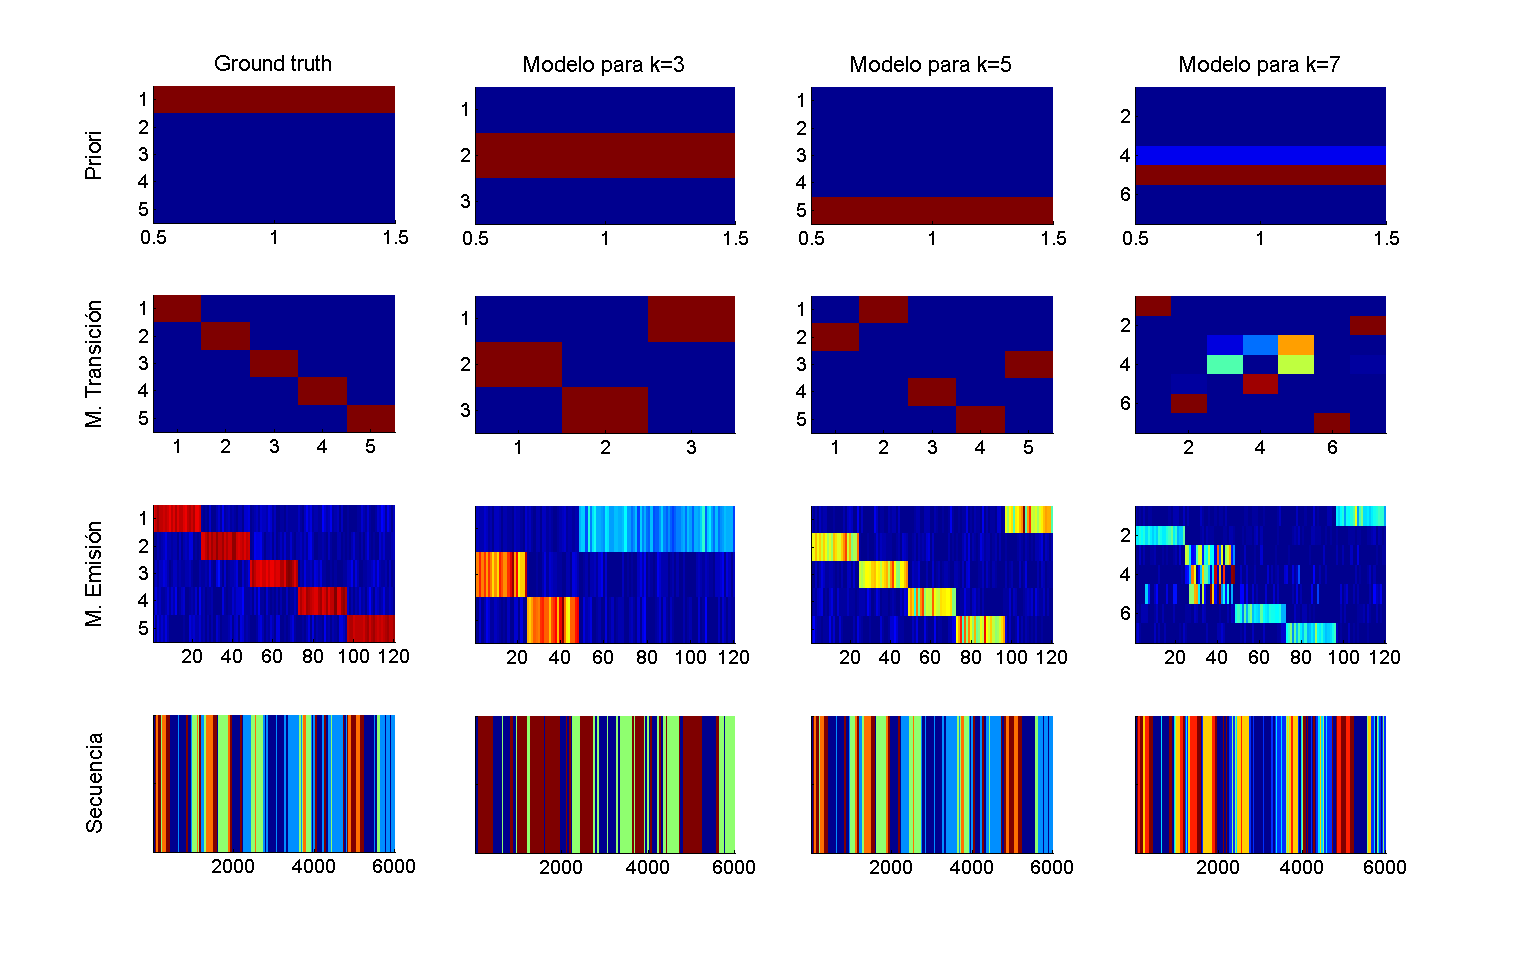
\includegraphics[height=0.65\textwidth]{gfx/pruebasg}
  \end{center}
\end{frame}

\begin{frame}{Synthetic data tests}
  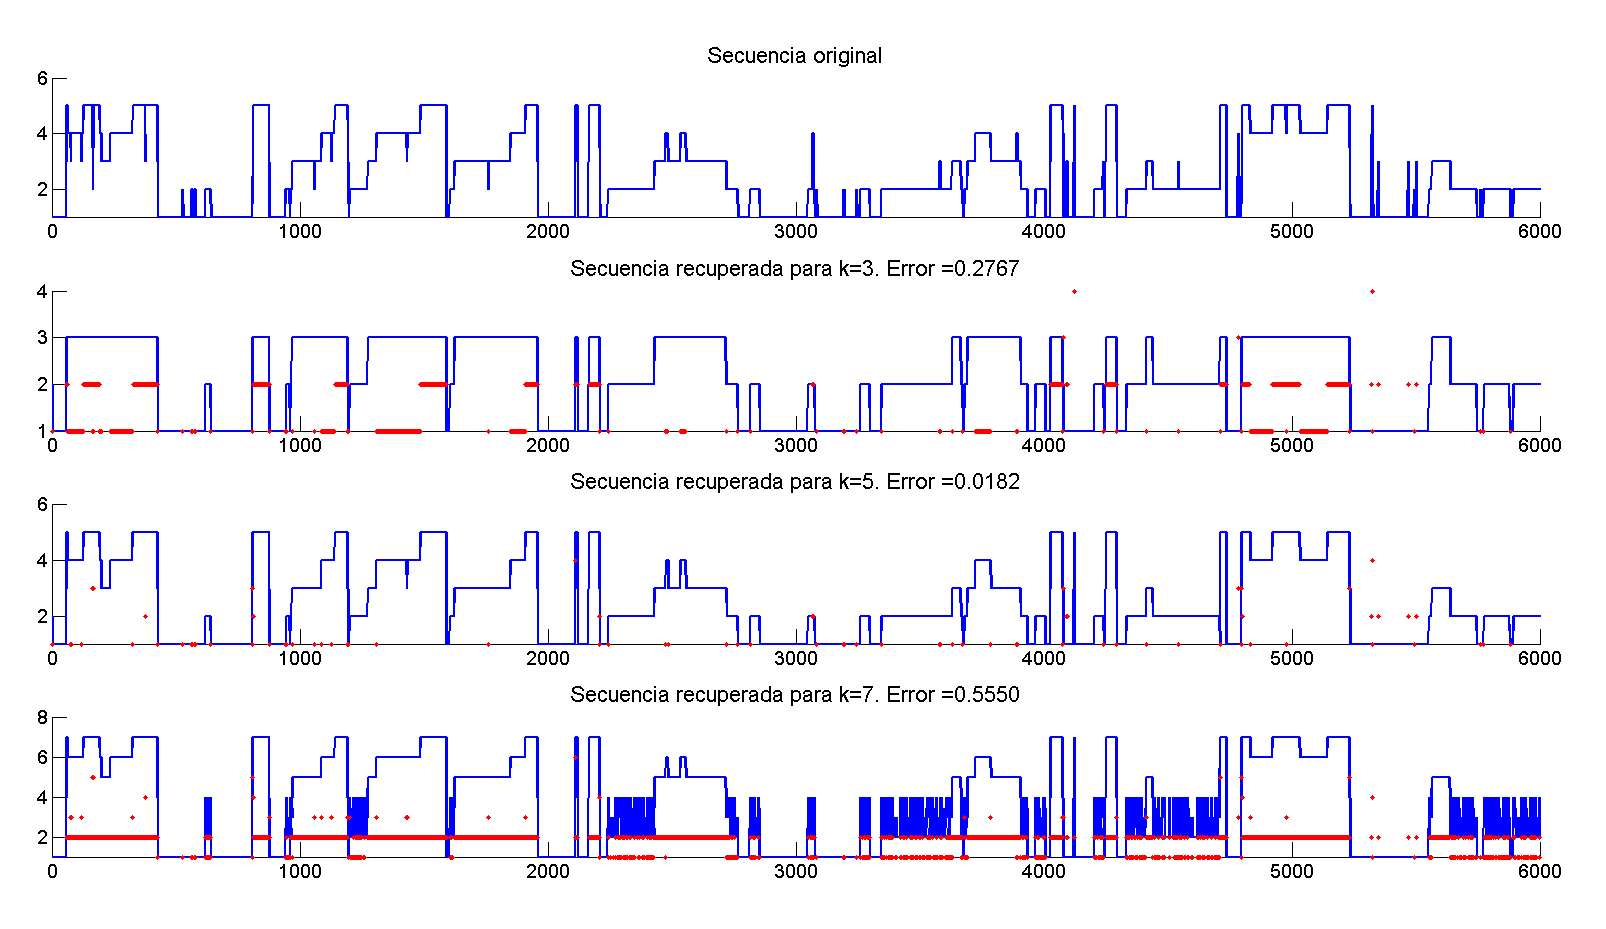
\includegraphics[height=0.6\textwidth]{gfx/pruebasg_}
\end{frame}

\section{Schedule}
\begin{frame}{Schedule}

\begin{center}
\begin{tikzpicture}[y=-\actheight,x=\actwidth]
    % First print a list of times.
    \foreach \nmonth/\Month in {2/February, 3/March, 4/April, 5/May, 6/June, 7/July}
        \node[anchor=north east] at (1, \nmonth) {\Month};

    \node[anchor=north] at (1.5, 0) {\large{Activities}};

    \node[entry={3.5}{2}] at (1.0, 2.4) {Tests for synthetic voice recordings};
    \node[entry={3}{2}] at (1.5, 3.5) {Analysis and comparision of results};
    \node[entry={2.0}{2}] at (1.0, 6.0) {Writing thesis};
  \end{tikzpicture}

\end{center}
\end{frame}

\section{Appendix}
\subsection{Reference material}

\begin{frame}{Reference material}
  
  \footnotesize {
  \begin{thebibliography}{10}
    
  \beamertemplatebookbibitems

  \bibitem{Bishop} 
  {L.R. Rabiner, B.H. Juang}
    \newblock \em{Fundamentals of speech recognition}
    \newblock Pearson Education India, 2008.
  
  \bibitem{Bishop}
    {C. M. Bishop.}
    \newblock \em{Pattern Recognition and Machine Learning}.
    \newblock Springer, 2006.
     
  \beamertemplatearticlebibitems
    
  \bibitem{Lawrence}
    {L.R. Rabiner}
    \newblock \em{A tutorial on hidden Markov models and selected 
      applications in speech recognition}
    \newblock Proceedings of the IEEE, 1989.

  \bibitem{Ryden}
    {T. Rydén.}
    \newblock \em{EM versus Markov chain Monte Carlo for Estimation of Hidden 
    Markov Models: A Computational Perspective}
    \newblock {Bayesian Analysis (2008) 3}, Number 4, p. 659-688
    
  \bibitem{Emily}
    {E.B. Fox, E.B. Sudderth, M.I. Jordan, A.S. Willsky.}
    \newblock \em{A sticky HDP-HMM with application to Speaker diarization}.
    \newblock {Annals of Applied Statistics}, 2011.
     
  \end{thebibliography}
  }
\end{frame}

\end{document}